% В этом шаблоне используется класс spbau-diploma. Его можно найти и, если требуется,
% поправить в файле spbau-diploma.cls
\documentclass{spbau-diploma}

\usepackage{graphicx,subcaption}
\usepackage{listings}
\usepackage[noend]{algpseudocode}
\usepackage{algorithm}
% \usepackage{algorithmicx}

\lstdefinelanguage{scala}{
  morekeywords={abstract,case,catch,class,def,%
    do,else,extends,false,final,finally,%
    for,if,implicit,import,match,mixin,%
    new,null,object,override,package,%
    private,protected,requires,return,sealed,%
    super,this,throw,trait,true,try,%
    type,val,var,while,with,yield},
  otherkeywords={=>,<-,<\%,<:,>:,\#,@},
  sensitive=true,
  morecomment=[l]{//},
  morecomment=[n]{/*}{*/},
  morestring=[b]",
  morestring=[b]',
  morestring=[b]"""
}
% ,frame=tlrb
\lstset{language=scala,basicstyle=\ttfamily,keywordstyle=\color{red},frame=single}

\renewcommand{\lstlistingname}{Пример кода}
\floatname{algorithm}{Алгоритм}


\begin{document}
% Год, город, название университета и факультета предопределены,
% но можно и поменять.
% Если англоязычная титульная страница не нужна, то ее можно просто удалить.
\filltitle{ru}{
    chair              = {Кафедра математических и информационных технологий},
    title              = {Отладчик типов языка программирования scala в IntelliJ IDEA},
    % Здесь указывается тип работы. Возможные значения:
    %   coursework - Курсовая работа
    %   diploma - Диплом специалиста
    %   master - Диплом магистра
    %   bachelor - Диплом бакалавра
    type               = {master},
    position           = {студента},
    group              = 604,
    author             = {Васильев Роман Алексеевич},
    % supervisorPosition = {д.\,ф.-м.\,н., профессор},
    % supervisor         = {Выбегалло А.\,А.},
    supervisorPosition = {},
    supervisor         = {Подхалюзин А.\,В.},
    reviewerPosition   = {},
    reviewer           = {Бреслав А.\,А.},
    chairHeadPosition  = {д.\,ф.-м.\,н., профессор},
    chairHead          = {Омельченко А.\,В.},
    % university = {САНКТ-ПЕТЕРБУРГСКИЙ АКАДЕМИЧЕСКИЙ УНИВЕРСИТЕТ},
    % faculty = {Центр высшего образования},
    % city = {Санкт-Петербург},
    % year             = {2013}
}
% \filltitle{en}{
%     chair              = {Department of Mathematics and Information Technology},
%     title              = {Empty subset as closed set},
%     author             = {Roman Vasiliev},
%     supervisorPosition = {professor},
%     supervisor         = {Amvrosy Vibegallo},
%     reviewerPosition   = {assistant},
%     reviewer           = {Alexander Privalov},
%     chairHeadPosition  = {professor},
%     chairHead          = {Alexander Omelchenko},
% }
\maketitle
\tableofcontents

% У введения нет номера главы
\section*{Введение}
Одним из наиболее популярных способов убедиться в корректности программы
является система типов.
Однако, также известно, что легче научится писать код на динамически типизируемых
языках программирования, чем на статически типизируемых.
Использование сложной системы типов ведет к сложности использования языка.

В языке программирования scala достаточно мощная система типов,
в которой используются такие понятия как: структурные типы, экзистенциальные
типы, f-bounded polymorphism.
И наличие таких продвинтутых контрукций может приводить к непониманию работы
системы проверки типов.
Сюда же можно отнести автоматический вывод типов, не указанных пользователем,
а также другие решения неявно приинимаемые компилятором.

В данной работе была предпринята попытка создать инструмент отладки типов для
языка scala.
Этот инструмент было решено делать на основе имеющегося плагина Scala Plugin к
среде разработки IntelliJ IDEA.

При работе с кодом scala, существенной часть работы среды
разработки занимают вычисление и проверка типов.
Поэтому отдельной задачей было, используя кодовую базу Scala Plugin,
уменьшить влияние на производительность плагина в целом.
В работе будет предложено решение основанное на макросах scala.

\section{Обзор}
\label{overview}

% В последнее время стало появлятся много новых языков программирования.
На данный момент scala является достаточно известным языком программирования
интерес к которому быстро растет.
Одной из важных особенностей scala является его желание элегантно объединить
объектно-ориентированное программирование с, набирающей популярность,
функциональной парадигмой.

В данной работе нас будет интересовать функциональная направленность scala.
К ней можно отнести: функции высших порядков, использование механизма
pattern matching или отдание предпочтения неизменяемым данным.
А также использование достаточно продвинутой системы типов.

Можно отметить следующие особенности системы типов scala:
\begin{itemize}
  \item Чтобы найти применение в промышленном программировании scala изначально
  создавался как язык совместимый с java.
  Это ведет к возможности использования классов java, а следовательно и типы
  из java являются допустимыми типами внутри scala.
  \item Унифицированная система типов. Все типы, начиная с типов функций или
  классов и заканчивая типами пришедшими из java входят в единую иерархию типов.
  Это отличается от того же java где ссылочные типы отделены от примитивных.
  Наибольшим типом в этой иерархии является \textbf{Any}, а наименьшим
  \textbf{Nothing}.
  \item Стандартным методом достижения переиспользования кода
  в функциональных языках является различного рода полиморфизм.
  В scala есть возможность как абстрагировать по типу части кода,
  например полиморфные методы, так и сами типы.
  К последнему случаю относятся конструкторы типов и параметризованные типы.
  В случае с конструктором типа есть возможность указать не только ограничения
  на передаваемые в него типы, но и вариантности.
  От них зависит как сводимость типовых аргументов скажется на
  сводимости полных типов.
  Например, \textbf{List[Derived]} сводится к \textbf{List[Base]}, если
  \textbf{Derived} сводится к \textbf{Base}.
  \item В scala можно абстрагироваться не только по полноценному типу,
  но и по конструктору типа.
  Это дает поддержку так называемых типов высших кайндов.
  \item Пожалуй, главной особенностью scala является механизм implicit у которого
  есть множество различных применений.

  Например, для метода часть его параметров можно пометить как неявные.
  В таком случае можно не передавать соответствующие аргументы явно.
  Компилятор сам выполнит поиск подходящих по типу неявных переменных,
  а после использует их в качестве аргументов.
  В комбинации с типами высших кайндов это позвоялет достичь ad-hoc полиморфизма,
  когда новая функциональность добавляется в класс без изменения самого
  класса.
  \item Также есть другие сущности пришедшие из теории типов:
  структурные типы, экзестенциальные типы, типы завиящие от пути...
\end{itemize}

В сложности системы типов есть как плюсы, так и минусы.
С одной стороны это повышает надежность кода кода за счет увеличения статичеких
проверок, приводя к, так называемой, типобезопасности.
Однако вместе с этим усложняется использование языка, а описание типовых
конструкций может стать громоздким.
Чтобы бороться с последним, компилятор предлагает не только выполнять проверки
типов, но выводить большинство типов самомтоятельно.

Часто нет необходимости явно указывать тип переменной, компилятор может
сам его вывести используя выражение в правой части.
Также может быть необязательно явно передавать типовые аргументы в полиморфную
функцию, компилятор может сам сделать неявное преобразование.

Однако все что связано с типобезопасностью компилятор делает неявно для пользователя.
А в случае несовпадения типов где-то, он просто выводит сообщение вида:
тип ожидался, тип найден.
И далеко не всегда просто понять в чем именно заключалась ошибка.
Нас будет интересовать возможность как проиллюстрировать процесс выведении типов,
так и процесс проверки типов в общем.

% Поэтому компилятор может дописывать типы за пользователя.
% Компилятор может выводить типы за пользователя, что особенно удобно с
% использованием лямбда-функций.
% Т.е. типы не указываются явно, а компилятор делает неявное преобразование.

% Хотелось бы исеть штуку, которая поможет с этим.

Как будет видно в дальнейших, инструменты связанные с отладкой типов часто
требуют специальные версии компилторов для своей работы.
Заметим что интегрированные среды разработки должны выполнять ту же работу по
работе с типами что и компилятор.
Действительно, нахождение семантических ошибок требует знания о типах.
Поэтому отладчик типов можно основывать не на компиляторе, а на ИСР.
А создание подобного инструмента в уже существующей среде, цель которой
облегчить написание кода, кажется разумной идеей.
Существуют две популярные ИСР для scala: Scala Plugin для intellij idea и
плагин scala IDE для eclipse.
Далее мы будем говорить про Scala Plugin в intellij idea.

\subsection{Отладчик типов для языка программирования OCaml}
\label{sec:ocaml}
В качестве примера отладчика типов рассморим проект Type Debugger для
языка программирования OCaml.

OCaml, как и большинство функциональных языков, использует мощную статическкую
типизацию, и, так же как в scala, компилятор берет на себя работу по выводу типов
не указанных явно.
Представим ситуацию, во время вывода типов компилятор OCaml находит противоречие:
одно подвыражение требует один тип, а другое предоставляет отличный.
В таком случае принятие решения о том какой тип на самом деле подразумевался
пользователем становится проблематичным.
Поэтому компилятор выбирает тип как-то и выдает сообщение об ошибке.

Type Debugger, призван помочь разработчикам на OCaml получать более
конструктивную информацию об ошибках во время вывода типов.
В ситуациях несовпадения типа он начинает задавать
вопросы пользователю, какой тип подразумевался у того или иного выражения.
По результатам ответов на эти вопросы Type Debugger понимает источник проблемы
и дает пользователю более конкрентые источник ошибки.

Отдельно стоит заметить, что для реализации подобной функциональности
Type Debugger для OCaml переиспользует код вывода типов в компиляторе OCaml.

Подобный проект создает прецедент существования отладчиков типов.

\subsection{Scala type debugger}
\label{sec:typeDebugger}

Возникает лаконичный вопрос - существует ли подобный инструмент для языка
программирования scala.
Ответ - да, существует.
Проект называется scala type debugger, и для ознакомления с ним можно посмотеть
репозиторий на github~\cite{type_debugger_github} и несколько
статей~\cite{type_debugger1}~\cite{type_debugger2}, одна из которых
написана в соавторстве с Мартином Одерски, создателем языка scala.

Цель этого инструмента анализировать проблемы связанные с типами.
Результатом его работы будет граф, где в вершинах записаны действия выполняемые
компилятором при типизации какого-то выражения, а также их результат.
По этому графу можно понять что делал компилятор для проверки типов и
в какой именно момент возникла ошибка.

Так как это прямой конкурент, то разберем что именно нас не устраивает в данном
проекте:
\begin{itemize}
  \item Так же как и Type Debugger для языка OCaml, scala type debugger
  переиспользует код компилятора scala.
  Для своей работы он требует специально инструментированную версию scalac.
  Это не очень удобно, нужно перенастраивать окружение под соответсвующую версию
  компилятора.
  При этом нашей целью является создать отладчик типов внутри Scala Plugin.
  Scala Plugin же занимается анализом кода самостоятельно и использует
  свое собственно внутреннее представление типов.
  Добавление некоего инструментированного компилятора создаст лишнюю зависимость.
  \item На момент написания работы репозиторий со scala type debugger не
  обновлялся в течение 5 лет.
  В статье~\cite{type_debugger1} написано о планах интегрировать его в eclipse.
  Но до сих пор этого не было сделано.
\end{itemize}

% Если же написать инструмент для анализа проверок типов основываясь исключительно
% на коде Scala Plugin, то для использования такого инструмента не будет никаких
% проблем.

\subsection{Show implicit parameters action}
\label{sec:showImplicit}

В заключение рассмотрим уже существующий в Scala Plugin инструмент, который
помогает пользователю разобраться в дейтсвиях компилятора.

В начале раздела уже описывалась работа механизм implicit параметров.
Существуют определенные правила поиска соответвствующих параметров,
но так как в коде это явно не указываются, часто этот механизм
может работать не вполне предсказуемо.
Ситуация осложняется существованием функций производящих неявные значения
используя другие неявные параметры и так далее.

Чтобы помочь облегчить работу с implicit парметрами в Scala Plugin существует
show implicit parameters action~\cite{show_implicit}.
Он в виде вложенных вкладок отрисовывает дерево, где узел - это функция требующая
неявные параметры, а лист - это неявная переменая.
Это дерео позволяет быстро навигироваться по коду.

Вообще говоря, многие процессы удобно визуализировать как деревья.
Забегая вперед, в данной работе будет использоваться такой-же стиль
представления информации как и у show implicit parameters action.

\subsection{Постановка цели}

На данный момент мы узнали достаточно чтобы сформулировать цель и задачи.

Цель:
реализовать отладчик процесса проверки типов в Scala Plugin.

Для этого можно выделить следующие задачи:
\begin{itemize}
  \item Инструментировать Scala Plugin для сбора данных о процессе работы с типами.
  \item Дать интерпретиацию приближенную к спецификации.
  \item Минимизировать влияние инструментации во время выполнения на оставшуюся
  часть плагина.
\end{itemize}

Теперь несколько замечаний про цели и задачи.

Несмотря на то что цель звучит достаточно общно, в
разделе~\ref{sec:implementation} будут конкретизированы процессы работы с типами
вызывающие интерес.

В разделе~\ref{sec:features} будет более подробно
рассказано почему в качестве способа сбора данных было выбрано именно
инструментирование исходного кода плагина.
Там же описана важность уменьшения влияния инструментации во время исполнения.

Также не получится целиком давать интерпретацию данных основываясь на спецификации
потому что плагин порою ей не следует.

Можно привести три случая непостредственной пользы подобного инструмента:
\begin{itemize}
  \item Понизить сложность вхождения.
  Как говоилось выше, у scala не самая простая система типов и разобраться
  в ней новичку может быть не просто.
  Данный инструмент позволит явно визуализировать работу с типами, которую
  производит Scala Plugin.
  \item Нетривиальные случаи.
  Хотя принцип работы будет основан на коде Scala Plugin а не scalac,
  существуют неочевидные ошибки не завязанные на специфике компилятора с которыми
  инструмент поможет спраиться.
  В разделе~\ref{sec:overloading} будет дан пример такой ситуации.
  \item Внутреннее использование.
  Для людей которые должны работать с внутренним устройством плагина это может
  дать представление о происходящем внутри без необходимости непосредственной
  отладки.
\end{itemize}

\section{Особенности реализации}
Здесь будет говориться как получать данные о работе того или иного процесса
внутри Scala Plugin.
Здесь и далее под процессом понимается последовательность выборов, принимаемых функциями и
классами внутри Scala Plugin, направленных на решение какой-то задачи.
Для начала нужно определиться, как именно будут получены эти данные.
Сделаем несколько наблюдений:

\begin{itemize}
  \item Чтобы не заниматься обратным анализом и не перереализовывать функциональность плагина,
  отвечающую за работу с типами, разумным выглядит переиспользовать уже существующую кодовую базу.
  \item Данные полученные о процессах нужно будет визуализировать.
  Поэтому хотелось бы их получать как полноценные объекты scala, а не как, скажем,
  набор снимков состояния стэка которые нуждаются в последующей обработке.
  Для этого формирование этих объектов должно быть отражено в коде рассматриваемых процессов.
  \item Scala Plugin написан на языке программирования scala.
  И хоть scala позициоирует себя как язык с функциональной направленностью,
  однако большая часть кода в плагине, необходимая для анализа процессов связанных с типами,
  написана в императивном стиле.
  То есть используются изменяемые состояния объектов, функции не всегда являются чистыми,
  а поток управления часто прерывается ключевым словом return.
  Поэтому во время получения данных было бы удобно пользоваться изменяемым состоянием.
\end{itemize}

В таких условиях разумной выглядит идея инструментировать фрагменты Scala Plugin,
отвечающие за интересующие нас процессы.
А именно, помещать в контекст выполнения процесса специальные объекты,
которык будут хранить данные о текущем состоянии процесса,
работа с которыми будет описана прямо в коде плагина, и которые
далее мы будем называть объектами инструментации.
Подробно это будет рассмотрено в разделе~\ref{sec:instrumentation}.

% todo рабочее
Однако, не стоит забывать, что Scala Plugin - это рабочее приложение
с большим количеством пользователь.
А код отвечающий за работу с типами, как минимум за сведение типов,
выполняется в плагине на каждом шагу.
Поэтому внесение дополнительных действий в этот код окажет пагубное воздействие
на производительность всего плагина.
Чтобы уменьшить воздействие инструментирования на процесс выполнения остального кода,
в данной работе принято решение использовать макросы.
Обзор возможностей макросов в scala приведен в разделе~\ref{sec:macroScala}.
Их применение к инструментированию на примере инструментированных функций
будет расммотрено в разделе~\ref{sec:macroScala}, а распространение на классы
в разделе~\ref{sec:macroClass}.

В конце будет раздел~\ref{sec:data}, посвященный формату хранения данных.

\subsection{Инструментирование}
\label{sec:instrumentation}

Здесь мы составим набор правил для использования инструментации так,
будто макросов нет.
Это позволит нам запускать код даже без них.
А в последующих разделах мы увидим что построенная система хорошо подходит
для анализа на уровне исходного кода.

Принцип, которым мы будем руководствоваться - инструментация должна быть опциональной.
Это означает что для запуска инструментированной версии кода нужно приложить
какие-то усилия, внешний код не обязан знать что возможно инструментирование.
Если ее не включить, влияние инструментирования на классы и функции будет
максимально снижено, поведение будет таким, каким было до инструментирования.

Попробуем представить как должно выглядеть инструментирование для, скажем, функции f.
Нам необходимо передать объект инструментации внутрь функции и дать знать,
нужно ли его использовать.
Это можно сделать или с помощью двух дополнительных параметров функции:
объекта и флага, или с помощью одного дополнительного параметра объекта,
который может принимать значение null.
Но в функциональном программировании есть более выразительное средство -
монада Option.
Значение по умолчанию None позволит не изменять уже существующие вызовы функции f.

\begin{lstlisting}[language=scala,basicstyle=\ttfamily,keywordstyle=\color{red}]
def f(..., instrumentation: Option[Instrumentation] = None)
\end{lstlisting}

Option и его функции высшего порядка такие как map и foreach автоматически дают нам
контекст, в котором мы можем выполнять любые необходимые действия,
в области видимости которого есть, непосредственно, объект инструментирования,
и которые игнорируются если Option оказался пуст.

\begin{samepage}
\begin{lstlisting}[language=scala,basicstyle=\ttfamily,keywordstyle=\color{red}]
instrumentation.foreach { i =>
  val a = computeA
  i.addInformation(a)
}
\end{lstlisting}
\end{samepage}

\textit{
Option для нас - это контекст, в котором живут все объекты и действия необходимые
для сбора данных. Покидать этот контекст им запрещено.
???
Написать Some как контекст.
}

Теперь поймем как хранить данные которые изменяются со временем.
Понятно что мы можем их хранить внутри объекта инструментации, и у нас нет другого
выхода если эти данные обновляются внутри вложенных вызовов функций.
Однако один и тот же объект инструментирования может появляться в множестве разных
частей программы и включение в него логики обработки промежуточных данных для
всех этих случаев может показаться избыточным.
Решением будет вынесение этих данных в изменяемую переменную.
Однако, мы хотим чтобы действия над этой переменной зависели от наличия объекта
инструментации.
В примере ниже показано как это сделать используя функцию map.

\begin{samepage}
\begin{lstlisting}[language=scala,basicstyle=\ttfamily,keywordstyle=\color{red}]
var intermediate = instrumentation.map(_ => Seq.empty[R])
for (i <- 0 to n) {
  val r = findResultFor(i)
  intermediate = intermediate.map(_ :+ r)
  doSomeStuff(r)
}
\end{lstlisting}
\end{samepage}

Таким образом мы явно связали переменную intermediate с контекстом instrumentation
в кототом и выполняется инструментация.
Аналогичным приемом можно воспользоваться если необходимо завести неизменяемы данные
вне контекста инструментации.
Это может понадобиться когда для вложенного вызова объект инструментации изменяется.

\begin{samepage}
\begin{lstlisting}[language=scala,basicstyle=\ttfamily,keywordstyle=\color{red}]
val inner = instrumentation.map(_.inner)
g(..., instrumentation = inner)
instrumentation.foreach(_.add(inner.get.data))
\end{lstlisting}
\end{samepage}

\textit{При возникновении новых сущностей связанных с
инструментированием, мы явно устанавливаем связь с уже существующими объектами.}

Разумным требованием кажется избегать влияния влияние интрументирования на
логику функции.
Но так ли это?
Рассмотрим в качестве примера проверку сводимости двух параметризованных типов.
Для сводимости одного типа к другому необходимо чтобы количества типовых параметров
совпадали и для каждой пары соответствущих типовых параметров выполнялось определенное соотношение.
При проверке этих соотношений достаточно дойти до первого ложного чтобы понять что
сводимость нет, что плагин и делает.
Однако в целях отладки было бы более информативно проверить все соотношения чтобы дать
пользователю более полную картину.

Таким образом возможность изменять поведение изначальной функции нам нужна.
Однако, есть версия что достаточно уметь делать две вещи:
изменять выбранную вертку исполнения в условных конструкциях при включенной
инструментировации, а также избегать прерывания потока исполнения ключевым словом return.

Основной идеей будет то что квантор всеобщности над пустым множеством всегда
верен, а квантор сущестования нет.
Таким образом мы можем использовать логику основанную на \textbf{существовании} объекта
в связке с \textbf{логическим или}, а также что-то для \textbf{любого} объекта
в связке с \textbf{логиеским и}.
Также заметим что любую конструкцию, тип которой Unit, такую как return,
мы можем записать через if (true).

Пример ниже иллюстрирует это.
В нем мы мы сначала игнорируем кэшированное значения с помощью проверки,
возвращающей false на непустом множестве.
Далее функции computeA и computeB из которых мы извлекаем данные.
Чтобы не прерываться после неудавшейся проверки conditionA, мы добавляем
условный оператор.
Если instrumentation пуст, то forall вернет true и поток исполнения прервется.
В обратном случае выполнится interrupt, который поднимет флаг остановки, а
forall вернет false и поток исполнения продолжится.
В конце мы с помощью exists проверяем был ли поднят флаг прерывания в процессе работы,
и если бы то возвращаем соответствующее значение.

\begin{samepage}
\begin{lstlisting}[language=scala,basicstyle=\ttfamily,keywordstyle=\color{red}]
val cached = cache.get(key)
if (cached != null && instrumentation.isEmpty) return cached

val conditionA = computeA(instrumentation = instrumentation)
if (conditionA)
  if (instrumentation.forall(!_.interrupt())) return false
val conditionB = computeB(instrumentation = instrumentation)
if (instrumentation.exits(_.interrupted())) return false
return conditionB
\end{lstlisting}
\end{samepage}

До этого момента мы говорили только о функциях.
Достаточно ли нам уметь работать только с ними?
Вообще говоря достаточно, но работать только с функциями неудобно.

Встречаются классы которые выступают как контейнеры функций.
Примерами могут служить классы MostSpecificUtil и MethodResolveProcessor.
Вместо того чтобы добавлять по параметру с объектом инструментации в каждый
метод, намного проще добавить один парметр в их конструкторы.
В будущем это усложнит задачу написания макроса.

\subsection{Макросы в scala}
\label{sec:macroScala}

Прежде чем говорить о макросах в scala, следует понять что имеется в виду под словом макрос.
Изначально, макрокоманда или макрос -- это символьное имя,
заменяемое при обработке исходного кода препроцессором на некоторый текст.
Наиболее известный пример макросов можно встретить в препроцессорах языков
программирования C и C++.

Подобные макросы работают по следующему механизму.
В начале пользователь описывает с помощью специального синтаксиса функцию,
которая примнимает в качестве параметров строковые константы, а возвращает текст,
в который могут быть подставлены значения этих параметров.
Перед компиляцией текста препроцессор проходит по тексту исходного кода и заменяет
вызовы этих функций на соответсвующие значения.
Как простые строки, без каких-либопроверок.
И только после этого, полученный текст отдается компилятору.

Использование макросов в scala контрастирует с вышеописанным подходом.
Главным отличием является то, что макросы в scala работают не со строками,
а с абстрактными синтаксическими деревьями, представляющими исходный код
программы.
Scala макросы пишутся на полноценном scala и являются функциями, принимающими
АСД фрагментов исходного кода и возвращающие АСД фрагментов которые нужно
сгенерировать.
То есть для того чтобы применить макрос к коду, компилятору требуется построить
АСД этого кода. Тем самым макросы не изменяют изначальный синтаксис, а лишь
преобразуют фрагменты кода.

Обычно эти макросы используют чтобы автоматически генерировать что-то для класса,
например сериализаторы.
И эти возможности предоставляет сам компилятор.
Однако существует плагин к компилятору Macro Paradise, который позволяет не
просто создавать новый код, но и заменять существующий.
Именно эту возможность мы и будем использовать для того чтобы снизитить влияние
кода инструментации на процесс исполнения.

Для того чтобы использовать Macro Paradise нужно создать специальную аннотацию,
которой должны быть помечены функции и классы код которых мы хотим изменить.
В класс этой аннотации должен быть добавлен код функции-генератора АСД.

Теперь поймем, чего мы хотим добиться используя кодогенерацию.
С одной стороны мы бы хотели полностью избавиться от кода связанного с инструментацией,
чтобы он никак не влиял на производительность плагина.
С другой стороны, эта инструментация добавлялась не просто так.
Выходом будет сгенерировать две копии каждой функции: одну с инструментацией,
другую без.
То же самое для классов.

Теперь опишем более подробно как именно это будет происходить.

\subsection{Макросы для функций}
\label{sec:macroFunction}

Сформулируем правила инструментирования полученные в
разделе~\ref{sec:instrumentation}:
\begin{enumerate}
  \item
  \label{itm:ins-constructor}
  Объект инструментирования передается явно как параметр функции или
  конструктора классов в монаде Option со значением по умолчанию None.
  \item
  \label{itm:ins-context}
  Действия связанные с инструментированием не должны покидать контекст
  инструментирования.
  \item
  \label{itm:ins-creating}
  Создание нового контекста инструментации происходит явно от другого,
  уже существующего, контекста инструментирования.
  Для этого подходит функция функция map.
  \item
  \label{itm:ins-logic}
  Для того чтобы влиять на первоначальную логику добавляются условные
  инвариантные для пустого контекста инструментизации условия.
\end{enumerate}


В этом разделе наша задача - по коду инструментированной функции f сгенерировать
пару новых функций \textbf{f} и \textbf{f\$I}.
Здесь \textbf{f} - это замена старой функции в которой будет удалено
все инструментирование.
\textbf{f\$I} - функция в которой оставлена инструментация.

Мы рассмотрим процесс генерации на очень концептуальном уровне.
И прежде всего нам потребуется вспомогательная функция
\textbf{GetInstrumentationNames} из алгоритма~\ref{alg:names}.

\textbf{Редактура!!!}

Эта функция нужна для обновления информации об именах связанных с инструментацией.
Теперь нам нужно найти новые созданные контексты инструментации внутри
тела \textbf{f}.
Это не сложно сделать, так как по пункту~\ref{itm:ins-creating} связь между ними
и старыми контекстами отслеживается в коде явно.
Имея множество имен, содержащих объекты инструментации мы можем находить новые
переменные созданные с помощью этих имен и функции map, а после добавлять их в
множество.

Теперь перейдем к рассмотрению генерации не инструментированной функции.

Функция \textbf{GetNonInstrumentedFunction} из алгоритма~\ref{alg:nonins}
выполняет искомую задачу.

По пункту~\ref{itm:ins-constructor} среди параметров этой функции должен быть
объект инструментации.
Допустим что нам известно его имя.
В первую очередь удаляем его.

Удалить действия связанные с инструментацией тоже не сложно.
Все они, по пункту~\ref{itm:ins-context}, находятся в соответствущих контекстах
связанных с именами объектов,а множество имен объектов у нас есть.
Заодно из кода вырезаются передачи этих объектов в вызовы функций.
Именно для этого требовалась явная передача аргументов.
Несмотря на то что можно было воспользоваться механизмом implicit,
нам бы потребовалась помощь компилятора чтобы находить передачу контекста
инструментирования.

Осталось наше влияние на первоначальную логику.
Но оно из пункта~\ref{itm:ins-logic} ограничивается использованием объектов
инструментации в условиях.
Чтобы вернуть все как было достаточно упростить все логические выражения,
подразумевая что используемые в них контексты инструментации пусты.
А также удалить условные конструкции, если они зависят только от объектов
инструментирования.

Логика генерации инструментированной функции намного проще.
Здесь нам достаточно изменить название самой функции и проследить чтобы все
вызовы используюшие инструментации были перенаправлены в инструментированный
код.

Таким образом избыточность создается только из-за увеличения количества функций
доступных для java virtual machine.

Также стоит заметить что применение аннотации к функции автоматически форсирует
нас использовать аннотации на всех вызванных внутри функциях, в которые мы передали
объекты инструментации.
Действительно, в инструментированной версии к этим функциям будет добавлен
суффикс \textbf{\$I} и код не скомпилируется если мы не позаботимся о наличии
соответсвующих функций.

\subsection{Макросы для классов}
\label{sec:macroClass}
Теперь перейдем к рассмотрению работы макро-аннотации класса.
Нашей задча остается прежней - по классу \textbf{C} сгенерировать пару:
инструментированный класс и неинструментированный.

Прежде всего заметим, что все относящееся к обработке инструментации внутри
функции также верно и для класса.
Здесь нас будут интересовать проблемы при создании классов, а также методы
их преодаления.
До этого момента все было хорошо.
Это связано с тем что функция не несет в себе состояния.
Она не участвует ни в каких иерархиях и для нее понятие инкапсуляции абсолютно.

Однако первая проблема с которой мы столкнемся будет не проблема наследования,
а сообщение Macro Paradise
"error: top-level class with companion can only expand into a block consisting
in eponymous companions".
Проблема заключается в следующем, Macro Paradise не добавляет новые имена в
верхний уровень видимости.
Единственное исключение - для класса можно сгенерировать его объект-компаньон.
В нашем же случае почти все классы вызывающие интерес лежат в верхнем уровне
видимости.

Что же, воспользуемся единственным исключением и вместо инструментированного
класса \textbf{C\$I} создадим инструментированный класс \textbf{\$I} который
будет лежать в объекте-компаньоне \textbf{C}.
Это решит проблему появления глобальных имен, и вызовы конструктора класса
\textbf{new C} в инструментированной версии будут перенаправляться
в \textbf{new C.\$I}.

Следующей проблемой будет - кто являются родителями \textbf{\$I}.
Кажется разумным выбрать тех же родителей что и у \textbf{C}.
Это правда пока не появляется функция принимающая \textbf{C} и вызываемая
внутри инструментрованного кода.
В качестве примера можно привести класс \textbf{MethodResolveProcessor}
который передает себя в метод \textbf{candidates} объекта-компаньона
через \textbf{this}.
Можно попытаться сгенерировать две копии метода \textbf{candidates},
но в таком случае становится сложнее отслеживать распространение контекста
инструментирования.
То что было описано в разделе~\ref{sec:instrumentation} перестает работать.
А за счет возможности импортировать имена из объектов (которой воспользовались
в плагине), без помощи компилятора даже нельзя понять, какие вызовы относятся
к тому что мы передали, а какие нет.

Остается наследование от \textbf{C}, чтобы номинальная система типов не могла
отличить от него \textbf{\$I}.

В начале поговрим о внутреннем состоянии класса.
Данные хранятся в переменных, изменяемых или неизменяемых.
А эти переменные могут быть или публичными, или приватными.
Часть из них объявлена в конструкторе.
Помимо этого у класса может быть инициализаци, которая может содержать побочные
эффекты.

Самое первое - нужно запретить инициализацию объекта.
С одной стороны из-за принципа инкапсуляции мы не можем проигнорировать
конструктор класса \textbf{C}.
С другой, если там должна была быть инструментация, то нам нужно перезапустить
конструктор в классе \textbf{\$I}, но уже с инструментацией.
Это может привести либо к несогласованности внутри класса, либо, если есть
побочные эффекты, к неожиданным внешним явлениям.
Самое простое - запретить общую инициализацию объекта, оставив передачу параметров.
Причем, оказывается что в нашем случае это не очень большое ограничение.
Как говорилось в начале раздела, нас интересуют классы являющиеся упаковками
функций.
В них отсутсвует секция инициализации и так.

Теперь нужно разобраться с переменными класса.
Если нет инициализации, то публичные переменные класса \textbf{C} мы можем
просто переиспользовать в методах класса \textbf{\$I}.
Приватные переменные же переменные класса \textbf{C} не покидают его область
видимости, поэтому их достаточно продублировать.
Единственным тонким моментом остаются переменные полчуаемые в конструкторе.
Естествееным желанием является скопировать эти переменные из конструктора
класса \textbf{C}, но в случае публичных переменных возникнет коллизия имен.
Чтобы обойти это ограничение, достаточно продублировать переменные в конструкторе
с лругими именами, а потом провести соответсвующие присвоения.

Последняя рассмотренная здесь сложность станет вызвана инкапсуляции.
Конкрентно, класс может вызвать super методы его родителя, но не может вызвать
их реализаии у прародителя.
Как это относится к нашему случаю?
Если в коде класса \textbf{C} найдется вызов метода его родителя,
а сам этот метод окажется перегружен, то к нас не будет возможности в
инструментированном коде сделать соответсвующий вызов.
А вышеупомянутый \textbf{MethodResolveProcessor} этим грешит.
Чтобы справится с этой проблемой приходится находить подобные методы и
вставлять в \textbf{C} их заместителей, которые и будут вызываны в \textbf{\$I}.

\textbf{Пример класс до, класс после.}

В случае с классом мы получаем избыточность сразу во многих местах:
дополнительный класс, дополнительные методы-заместители, возможно изменение
модификатора приватный на защищенный для наследования.
Это усложняет работу виртуальной машины и может делать невозможными некоторые
отимизации.

На этом часть связанная с инструментированием кода и макросам заканчивается.
Все вышеописанное можно посмотреть в коде плагина.
Логика обработки АСД находится в
\textbf{org.jetbrains.plugins.scala.macroAnnotations.uninstrumentedMacro}.
Сама же аннотация называется \textbf{uninstrumneted}, она принимает в качестве
аргумента название параметра, соответсвующего объекту инструментации.
Всего в проекте потребовалось использовать 28 таких аннотаций.

\subsection{Сохраненные данные и визуализация}
\label{sec:data}

Здесь мы немного поговорим о визуализации накопленных данных,
и о том в каком виде эти данные удобно хранить.

Было решено визуализировать данные в виде вложенных вкладок.
Для этого было две причины.
Во первых, сходимость типов удобно иллюстрировать деревьями вывода,
о чем будет рассказано в разделе~\ref{sec:conformance}.
Во вторых, можно ориентироваться на show implicit parameters action
в scala plugin из раздела~\ref{sec:showImplicit}.
Там выбор необходимых implicit параметров иллюстрировался тоже с помощью
вложенных вкладок и это было удобно.

Далее, заметим что для описания древовидных структур, рекурсивных или нет,
прекрасно подходят алгебраические типы данных, столь популярные функциональном
программировании.
Подробнее про них можно почитать в \cite{algebraic_data}.
В scala есть подходящий для такой абстракции механизм, называемый case class.
Именно с помощью него мы и будем хранить все необходимые данные.
А во время визуализации решение что именно нужно отрисовать будет приниматься
с помощью механизма pattern matching.

\textbf{Если нужно, добавить пример каких-то классов.}

\section{Реализация}
\label{sec:implementation}

В этом разделе наше внимание сместится на осбенности реализации процессов
связанных с типами в Scala Plugin и особенности их инструментирования.
\textbf{Так как конечной целью является визуализация работы этих процессов, то
хочется максимально опираться на стандарт языка, которым является спецификация
scala \cite{scala_spec}.}
Мы проследим как соответсвующие понятия из спецификации переносятся в Scala Plugin.
А там где это не возможно будет явно указано на расхождение в реализации плагина и
спецификации.
Так-же будет указано как визуализируется каждый процесс.

% Реализация в плагине в плагине
% Смысл в последующей визуализации
% Хочется сделать С уважением к спецификации
% Однако не везде это возможно сделать
% Где можно сделаем
% Везде будет указано расхождение

До этого момента, когда мы говорили о работе плагина, то использовали
нейтральное слово процесс.
Теперь нужно вспомнить, что изначальной задачей было явно визуализировать
работу связанную с типами, которую плагин делает неявно.
Архитектура части плагина связанной с типами будет
рассмотрена в разделе \ref{sec:arch}.
Перечислим интересующие нас процессы.

Базовым процессом является сравнение двух типов.
В спецификации для этого вводятся три понятия: эквивалентность типов, сводимость
типов и слабая сводимость типов.
Эквивалентность означает что один тип мы в любом контексте можем заменить другим
типом, и это отношение наиболее понятно интуитивно.
Сводимость типов намного более интересна и используется во всех других процессах.
Ее мы рассмотрим в разделе~\ref{sec:conformance}.
Там же будет описание слабой сводимости, а также будет разобрано представление
типов в Scala Plugin и их отличия от типов описанных в спецификации scala.

Следующим интересующим нас процессом будет вывод типов.
Важно что вывод типов в плагине и в спецификации осуществляется по разному.
Подробно об этом будет написано в разделе~\ref{sec:infer}

Последний процесс, следующий из вывода типов - это разрешение перегрузок функций.
Действительно, типовые переменные появляются в вызовах полиморфных
функций и их неявный вывод актуален для конкретного вызова.
А так как в scala присутствуют перегрузки функций, то прежде всего нужно
разрешить символ на котором были вызваны аргументы.
Процесс разрешения перегрузок будет рассмотрен в разделе~\ref{sec:overloading}.

Отдельного упоминания заслуживает механизм implicit.
В данной работе не затрагивались неявные преобразования и неявные параметры.
В рамках Scala Plugin уже существуют ShowImplicitParametersAction, показывающий
неявно передаваемые параметры, и GoToImplicitConversationAction, помогающий
в работе с неявными преобразованиями.
Так же в данной работе не освященна работа с динамическими типами.

\subsection{Архитектура Scala Plugin}
\label{sec:arch}

\begin{figure}[t]
\centering
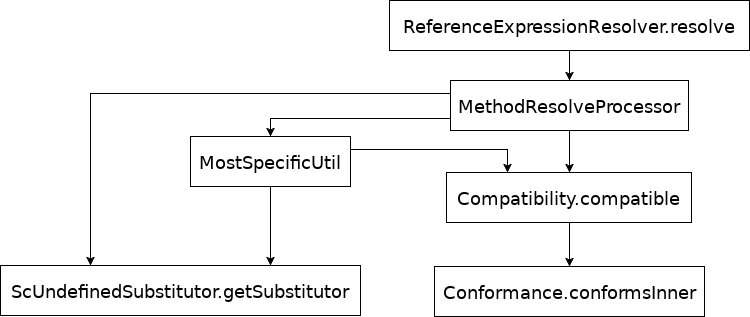
\includegraphics[width=\textwidth]{img/call-graph}
\caption{Граф вызовов}
\label{fig:callGraph}
\end{figure}

Как говорилось в начале главы~\ref{sec:implementation}, нас будут интересовать
процессы сведения типов, выведения типов и выбора перегрузки функции.
Все эти процессы можно проилюстрировать на вызове полиморфной функции.
Для начала рассмотрим как он будет обрабатываться плагином с
точки зрения архитектуры.
На рисунке~\ref{fig:callGraph}, несколько упрощенно, показан граф вызовов
такой обработки.
Мы явно будем указывать классы, основные и вспомогательные функции в которых
использовалась аннотация uninstrumented.
Это нужно чтобы понять куда именно добавлялась инструментация.
% основываясь на интересующих нас процессах

\textbf{Улучшить введение.}
Представим что у нас есть символ \textbf{f} и аргументы
\textbf{e1} ,..., \textbf{en}.
Для проверки этого применения будет вызван метод \textbf{resolve} объекта
\textbf{ReferenceExpressionResolver}.
Это и будет точкой входа.
Аннотировано uninstrumented:
\begin{itemize}
  \item \textbf{ReferenceExpressionResolver.resolve}
\end{itemize}
% Здесь только к методу \textbf{resolve} будет добавлена аннотация uninstrumented.

Далее с помощью класса \textbf{MethodResolveProcessor} будет осуществлен
поиск кандидатов обладающих таким же именем как \textbf{f}.
\textbf{MethodResolveProcessor} будет хранить множество кандидатов и
результаты применения соответсвующих кандидатов к аргументам.
Также там находится часть логики по фильтрации кандидатов, более подробно о которой
будет написано в разделе~\ref{sec:overloading}.
Аннотировано uninstrumented:
\begin{itemize}
  \item класс \textbf{MethodResolveProcessor}
  \item \textbf{MethodResolveProcessor.problemsFor}
  \item \textbf{MethodResolveProcessor.candidates}
\end{itemize}
% Аннотация uninstrumented была добавлена к самому классу
% \textbf{MethodResolveProcessor}, а также к вспомогательным методам
% объекта-компаньона \textbf{problemsFor} и \textbf{candidates}.

Для каждого кандидата нужно проверить, возможно ли вызвать его с такими аргументами.
Инструменты для этого находятся в классе \textbf{Compatibility}.
Омновная часть кода здесь - это перебор разных конструкций Scala Plugin,
описывающих исходный код, а также способов применения к ним аргументов.
Например, разбор таких случаев как передача аргумента по имени или параметры со
значением по умолчанию.
Аннотировано uninstrumented:
\begin{itemize}
  \item \textbf{Compatibility.checkConformance}
  \item \textbf{Compatibility.checkConformanceExt}
  \item \textbf{Compatibility.compatible}
\end{itemize}
% Здесь аннотация uninstrumented добавлена к методам объекта
% \textbf{checkConformance}, \textbf{checkConformanceExt} и \textbf{compatible}.

Для проверки двух типов используется интерфейс \textbf{Conformance}.
У этого интерфейса две реализации: одна для системы типов scala, другая для
системы типов dotty \cite{dotty}, нового поколения языка scala.
В обоих случаях метод \textbf{conformsInner} возвращает пару: возможна ли
сходимость и набор ограничений на абстрактные типы при которых сходимость
возможна.
Про процесс сходимости написано в разделе~\ref{sec:conformance}.
Аннотировано uninstrumented:
\begin{itemize}
  \item \textbf{Conformance.conformsInner}
  \item \textbf{Conformance.computable}
  \item \textbf{Conformance.checkParameterizedTypes}
  \item \textbf{Conformance.addParam}
  \item \textbf{Conformance.addArgedBound}
  \item класс \textbf{Conformance.LeftConformanceVisitor}
\end{itemize}
% Здесь аннотации uninstrumented применяются к методам
% \textbf{conformsInner}, \textbf{computable}, \textbf{checkParameterizedTypes},
% \textbf{addParam}, \textbf{addArgedBound}, а также к
% классу \textbf{LeftConformanceVisitor}.

Далее необходимо проверить что ограничения полученные на предыдущем шаге
возможно разрешить.
Для этого есть интерфейс \textbf{ScUndefinedSubstitutor}.
Его реализуют \textbf{ScUndefinedSubstitutorImpl} и
\textbf{ScMultiUndefinedSubstitutor}.
Отличие одной реализации от другой состоит в том, что
\textbf{ScUndefinedSubstitutorImpl} хранит только один набор ограничений, в
то время как \textbf{ScMultiUndefinedSubstitutor} хранит сразу несколько.
Это может понадобится если существует более одного способа добиться сводимости
типов. Конкретно это используется для составных типов.
Заметим, что разрешение ограничений на абстрактные типы - это и есть вывод типов.
Больше информации можно получить в разделе~\ref{sec:infer} о выводе типов.
Аннотировано uninstrumented:
\begin{itemize}
  \item \textbf{ScUndefinedSubstitutor.addLower}
  \item \textbf{ScUndefinedSubstitutor.addUpper}
  \item \textbf{ScUndefinedSubstitutor.getSubstitutorWithBounds}
  \item \textbf{ScUndefinedSubstitutor.getSubstitutor}
\end{itemize}
% Аннотация uninstrumented используется методах \textbf{addLower},
% \textbf{addUpper}, \textbf{getSubstitutorWithBounds}, а также \textbf{getSubstitutor}.

Интересно заметить, что пара \textbf{Compatibility} и
\textbf{ScUndefinedSubstitutor} образуют что-то вроде алгоритма
Хиндли-Милнера \cite{hindley–milner}.

Остался класс \textbf{MostSpecificUtil}.
Он нужен если после всех проверок сделанных \textbf{MethodResolveProcessor}
осталось больше одного кандитата.
В таком случае требуется найти наиболее специфичного кандитата.
Именно этим \textbf{MostSpecificUtil} и занимается.
Подробнее в разделе~\ref{sec:overloading}.
Аннотировано uninstrumented:
\begin{itemize}
  \item класс \textbf{MostSpecificUtil}.
\end{itemize}
% С помощью uninstrumented аннотируется только сам класс
% \textbf{MostSpecificUtil}.

% Все это было инструментровано для сбора дополнительных данных.
Всего в проекте потребовалось использовать 28 аннотаций uninstrumented.
Стоит заметить что граф вызовов сильно упрощен для улучшения понимания.
На самом деле по разным причинам все вызывают почти всех.

% Повсюду куча сравнений...\textbf{MethodResolveProcessor} \textbf{Compatibility}


\subsection{Проверка сводимости типов}
\label{sec:conformance}

В этом разделе будет рассмотрен процесс сводимости типов, будут описаны
структуры отвечающие за типы в Scala Plugin, а также дано стравнение типов
Scala Plugin и типов описанных в спецификации scala.

В спецификации scala сводимость вводится как транзитивное замыкание над
набором аксиом и правил вывода.
Это достаточно формальное определение.
Если следовать ему, то любое сведенение типов является некоторым доказательством.
А чтобы убедить кого-то в этом сведении, нужно предоставить корректное дерево
вывода.
Так что алгоритм, который занимается проверкой сводимости двух типов - это
в некотором роде система автоматического доказательства.
Существет множество систем автоматического доказательства \cite{automata},
однако наша логика слишком проста чтобы использовать, например, coq.
Так же стоит отметить, что слабая сводимость - это просто расширение набора
правил вывода для типов наследующихся от AnyVal.

В Scala Plugin для проверки сводимости на вход подаются два типа,
далее мы будем называть их левым и правым, задача свести правый к левому.
После этого для левого типа запускается шаблон посетитель, во время которого
тип конкретизируется, а после происходят проверки основанные на правилах
вывода.
Во время этих проверок посетитель может запускаться еще и для правого типа.
В самом конце идет проверка, является ли правый тип наследником левого.
Подробнее это можно посмотреть в объекте \textbf{Conformance}.

Стоит отметить что с одной стороны такой подход достаточно прост для анализа.
Однако с другой стороны в нем много избыточности, например, постоянные повторяения
одной и той логики для правого и левого типов.
Так же присутствуют постоянные проверки типов на Any и Nothing.
В первый раз они встречаются на самом верхнем уровне, а после проверки на них
присутствуют в самых неожиданных местах.
В коде можно встретить \textbf{java.lang.Object}, хотя упоминания о
нем в системе типов scala кажется странным.
Забегая вперед, одним из типов в Scala Plugin является JavaArray.
В scala для абстракции над массивом существует класс \textbf{scala.Array} и на
уровне типов это сводится к частному случаю параметризованного класса.
Отдельная сущность для массива влечет дублирование кода для параметризованных
типов, в котором и так очень много повторений.
Все это сильно повышает неоднородность кода.

Теперь поговорим про визуализацию сводимости типов.
Как говорилось в начале главы~\ref{sec:implementation} сведение типов является
базовым процессом, который встречается постоянно и его наглядная визуализация
очень важна.
В качестве представления дерева мы будем использовать вложенные вкладки,
которые имеют древовоидную структуру.
Это достаточно естественное решение, учитывая что само сведение является
деревом вывода.

Узлы дерева будут делиться на два типа:
\begin{itemize}
  \item Узлы отношения.
  В этих узлах записано что рассматриваемые в данный момент
  типы должны состоять в каком-то отношении.
  Это может быть либо правда, либо нет.
  Как пример, можно рассмотреть код~\ref{lst:conformance}.
  В нем мы объявляем отношение сводимости. Оно определено для двух типов:
  правого и левого.
  Для того чтобы оно было истинным, должно быть выполнено хотя бы одно из
  условий сводимости.
  \item Узлы условий.
  Эти узлы символизируют собой аксиомы и правила вывода введенные в спецификации
  scala.
  Часть условий может иметь сложную структуру и требовать выполнения каких-то
  отношений, из-за чего структура получается рекурсивной.
  В коде~\ref{lst:condition} находится интерфейс условия для сводимости.
\end{itemize}


\begin{lstlisting}[caption={Узел условия},label={lst:condition}]
sealed trait CCondition {
  def satisfy(ctx: RelationContext): Boolean
}
\end{lstlisting}

\begin{lstlisting}[caption={Узел отношения},label={lst:conformance}]
case class Conformance(left: ScType, right: ScType,
           conditions: Seq[CCondition]) extends Relation {
  override def satisfy(ctx: RelationContext): Boolean =
    conditions.exists(_.satisfy(ctx))
}
\end{lstlisting}

Все по заповедям раздела~\ref{sec:data}.

В обоих случаях передается контекст.

В ходе работы собираются условия.
после рекурсивных вызовов полученные условия объединяются в отношения.
После этого мы получаем уже готовую для визуализации структуру.  

\textbf{Картинка во вложении.}


Value Types

Non-Value Types

\subsubsection{Singleton Types}
\subsubsection{Type Projection}
dot calculus \cite{dot_calculus}
\subsubsection{Type Designators}
\subsubsection{Parameterized Types}
\subsubsection{Compound Types}
\subsubsection{Existential Types}
\subsubsection{Method Types}
\subsubsection{Polymorphic Method Types}
Типы высших кайндов - куда-то
\subsubsection{Type Constructors}
Запустить, посмотреть во что выльется.

\subsection{Вывод типов}
\label{sec:infer}

Вывод типов локальный.

В спекцификации вывод типов так-то.
В плагине абсолютно иначе.

Информация про выведенные типы попадает обратно в сходимость.
\subsection{Разрешение перегрузок функций}
\label{sec:overloading}


% У заключения нет номера главы
\section*{Заключение}

В данной работе были рассмотрены процессы, связанные с проверкой типов в
языке scala, выполнение которых производится неявно для пользователя.
Были рассмотрены различные инструменты, помогающие пользователям решать
проблемы, возникающие из-за сложности систем типов разных языков.

Основываясь на спецификации scala, в Scala Plugin был добавлен инструмент,
позволяющий явно визуализировать эти процессы.
Реализация производилась с использованием инструментирования.
Для снижения влияния на производительность была предложена методика
инструментирования с возможной последующей автоматической обработкой на
уровне исходного кода.
Был предложен алгоритм на основе макросов, позволяющий использовать
инструментирование, не замедляя при этом основную работу плагина.
% Также был рассмотрен пример такой обработки на примере макросов в scala.

Код можно посмотреть в репозитории на
github~\footnote{\url{https://github.com/nizshee/intellij-scala}}.

% Несмотря на
% Я бы не советовал в продакшн, много избыточного кода.

\setmonofont[Mapping=tex-text]{CMU Typewriter Text}
\bibliographystyle{ugost2008ls}
\bibliography{diploma}

\stepcounter{section}
\hfill ПРИЛОЖЕНИЕ А
\begin{center}
  \textbf{Алгоритмы обработки инструментрованных функций}
\end{center}
\markboth{\MakeUppercase{}}{}
\addcontentsline{toc}{section}{Приложение А. Алгоритмы обработки инструментрованных функций}

\begin{algorithm}
\caption{Обновление информации о контекстах инструментизации}\label{alg:names}
\begin{algorithmic}[1]
\Function{UpdateInstrumentationNames}{$codeBlock, previousNames$}
  \State $names \gets previousNames$
  \For {$expr \gets$ выражения внутри $codeBlock$}
    \If {$expr$ объявление символа $n$ с использованием $names$}
      \State $names \gets names$ добавить $n$
    \ElsIf {$expr$ объявление символа $n$}
      \State $names \gets names$ убрать $n$
    \EndIf
  \EndFor
  \State \Return names
\EndFunction
\end{algorithmic}
\end{algorithm}

\begin{algorithm}
\caption{Генерация неинструментированной функции}\label{alg:nonins}
\begin{algorithmic}[1]
\Function{GetNonInstrumentedFunction}{$func, parameterName$}
  \State удалить $parameterName$ из сигнатуры функции $func$
  \State $codeBlock \gets$ получить тело $func$
  \State $HandleNonInstrumentedBlock(codeBlock, parameterName)$
\EndFunction

\Function{HandleNonInstrumentedBlock}{$codeBlock, previousNames$}
  \State $names \gets UpdateInstrumentationNames(codeBlock, previousNames)$
  \For {$expr \gets$ выражения внутри $codeBlock$}
    \If {$expr$ это условние в котором есть только элемент из $names$}
      \State заменить все условное выражение на одну из ветвей
    \ElsIf {$expr$ это условие содержащее элемент из $names$}
      \State упростить условие, исключив из него элементы из $names$
    \ElsIf {$expr$ это вызов с использованием элемента из $names$}
      \State удалить аргументы связанные с $names$ из вызова
    \ElsIf {$expr$ основан на элементе из $names$}
      \State удалить $expr$
    \ElsIf {$expr$ это новый блок кода}
      \State $HandleInstrumentedBlock(expr, names)$
    \ElsIf {$expr$ содержит элемент из $names$}
      \State \Return ошибка
    \EndIf
  \EndFor
\EndFunction
\end{algorithmic}
\end{algorithm}

\begin{algorithm}
\caption{Генерация инструментированной функции}\label{alg:ins}
\begin{algorithmic}[1]
\Function{GetInstrumentedFunction}{$func, parameterName$}
  \State добавить к названию функции $func$ суффикс $\$I$
  \State $codeBlock \gets$ получить тело $func$
  \State $HandleInstrumentedBlock(codeBlock, parameterName)$
\EndFunction

\Function{HandleInstrumentedBlock}{$codeBlock, previousNames$}
  \State $names \gets UpdateInstrumentationNames(codeBlock, previousNames)$
  \For {$expr \gets$ выражения внутри $codeBlock$}
    \If {$expr$ это вызов с использованием элемента из $names$}
      \State добавить к имени символа суффикс $\$I$
    \ElsIf {$expr$ это новый блок кода}
      \State $HandleNonInstrumentedBlock(expr, names)$
    \EndIf
  \EndFor
\EndFunction
\end{algorithmic}
\end{algorithm}

\end{document}
